\documentclass{article}
\usepackage{graphicx, amssymb, amsmath, mathtools}
\graphicspath{{Images/}}


\setlength{\oddsidemargin}{0in}
\setlength{\textwidth}{6.5in}
\setlength{\topmargin}{-.55in}
\setlength{\textheight}{9in}
\pagestyle{empty}



\newcommand{\minimize}[0]{\text{minimize}}

\title{Optimization HW 7}
\author{Michael Nameika}
\date{April 2023}

\begin{document}

\maketitle

\section*{Section 11.5 Problems}
\textbf{1.} Consider the problem
\[\text{minimize} \:\:\:\:\: f(x_1, x_2) = (x_1 - 2x_2)^2 + x_1^4\]
\begin{itemize}
    \item[(i)] Suppose a Newton's method with a line search is used to minimize the function, starting from the point $x = (2,1)^T$. What is the Newton search direction at this point?
    \newline\newline
    Recall that the Newton search direction is given by solving the linear system
    \[\nabla^2f(x_k)p_k = -\nabla f(x_k)\]
    For our problem, we find the following for the gradient and Hessian of $f$:
    \begin{align*}
        \nabla f(x_1,x_2) &= \begin{pmatrix*}[c]
            2(x_1 - 2x_2) + 4x_1^3\\
            -4(x_1 - 2x_2)
        \end{pmatrix*}\\ \\
        \nabla^2f(x_1,x_2) &= \begin{pmatrix*}[c]
            2 + 12x_1^2 & -4\\
            -4 & 8
        \end{pmatrix*}
    \end{align*}
    and with $x_0 = (2,1)^T$, we have
    \begin{align*}
        \nabla f(x_0) &= \begin{pmatrix*}[r]
            32\\
            0
        \end{pmatrix*}\\
        \\
        \nabla^2f(x_0) &= \begin{pmatrix*}[r]
            50 & -4\\
            -4 & 8
        \end{pmatrix*}
    \end{align*}
    Then we find 
    \[p_0 = \begin{pmatrix*}[r]
        -2/3\\
        -1/3
    \end{pmatrix*}\]

    \item[(ii)] Suppose a backtracking line search is used. Does the trial step $\alpha = 1$ satisfy the sufficient decrease condition for $\mu = 0.2$? For what values of $\mu$ does $\alpha = 1$ satisfy the sufficient decrease condition?
    \newline\newline
    Recall the sufficient decrease condition:
    \[f(x_k + \alpha_kp_k) \leq f(x_k) + \mu\alpha_kp_k^T\nabla f(x_k)\]
    For $\mu = 0.2$, $\alpha = 1$, and $p_k$ given by $p_0$ in part (i), we find the following:
    \begin{align*}
        f(x_k + \alpha_kp_k) &= f(4/3, 2/3) = \frac{256}{81}\\
        f(x_k) + \mu\alpha_kp_k^T\nabla f(x_k) &= 16 + (0.2)(1)(-2/3,-1/3)(32,0)^T\\
        &= \frac{176}{15}
    \end{align*}
    Observe that $\frac{256}{81} \approx 3$ and $\frac{176}{15} \approx 11$, so the sufficient decrease condition is satisfied for $\mu = 0.2$. Now we wish to find all values of $\mu$ such that the sufficient decrease condition is satisfied. That is, we must solve 
    \[f(x_k + \alpha_kp_k) \leq f(x_k) + \mu\alpha p_k^T\nabla f(x_k)\]
    for $\mu$ with the added condition that $\mu > 0$. Using $x_k = (2,1)^T$, $p_k = (-2/3,-1/3)^T$, $\alpha_k = 1$, we find
    \begin{align*}
        \mu &\leq \frac{256/81 - 16}{-64/3} \\
        &= \frac{65}{108}\\
    \end{align*}
    and so The values of $\mu$ that the trial step $\alpha = 1$ satisfies the decrease condition are
    \[0 < \mu \leq \frac{65}{108}\]
    \newline
\end{itemize}
\textbf{2.} Let
\[f(x_1,x_2) = 2x_1^2 + x_2^2 - 2x_1x_2 + 2x_1^3 + x_1^4\]
\begin{itemize}
    \item[(i)] Suppose that the function is minimized starting from $x_0 = (0,-2)^T$. Verify that $p_0 = (0,1)^T$ is a direction of descent.
    \newline\newline
    Recall that $p_0$ is a direction of descent in case
    \[p_0^T\nabla f(x_0) < 0\]
    First, let us find $\nabla f(x_0)$. For the gradient we have
    \[\nabla f(x_1,x_2) = \begin{pmatrix*}[c]
        4x_1 - 2x_2 + 6x_1^2 + 4x_1^3\\
        2x_2 - 2x_1
    \end{pmatrix*}\]
    and so
    \[\nabla f(x_0) = \begin{pmatrix*}[r]
        4\\
        -4
    \end{pmatrix*}\]
    and we have
    \begin{align*}
        p_0^T\nabla f(x_0) &= (0,1)\begin{pmatrix*}[r]
            4\\
            -4
        \end{pmatrix*}\\
        &= -4 < 0
    \end{align*}
    So $p_0 = (0,1)^T$ is a descent direction of $f$ at $x_0 = (0,-2)^T$.
    
    \item[(ii)] Suppose that a line search is used to minimize the function $F(\alpha) = f(x_0 + \alpha p_0)$, and that a backtracking line search is used to find the optimal step length $\alpha$. Does $\alpha = 1$ satisfy the sufficient decrease condition for $\mu = 0.5$? For what values of $\mu$ does $\alpha = 1$ satisfy the sufficient decrease condition?
    \newline\newline
    Recall again the sufficient descent condition:
    \[f(x_0 + \alpha p_0) \leq f(x_0) + \mu\alpha p_0^T\nabla f(x_0)\]
    Evaluating the right-hand side, we find
    \begin{align*}
        f(x_0) + \mu\alpha p_0^T\nabla f(x_0) &= 4 + (0.5)(1)(-4)\\
        &= 2
    \end{align*}
    and the left hand side:
    \begin{align*}
        f(x_0 + \alpha p_0) = f(0,-1) = 1
    \end{align*}
    Clearly, $1 \leq 2$, so the sufficient decrease condition is satisfied. Now we wish to find the values of $\mu$ that satisfy the sufficient decrease condition for $\alpha = 1$. Well, from above, we can see we wish to find $\mu$ that satisfy (with the added condition that $\mu > 0$
    \[1 \leq 4 - 4\mu\]
    Clearly, we require $\mu \leq 3/4$. Then the values of $\mu$ that satisfy the sufficient decrease condition are
    \[0 < \mu \leq \frac{3}{4}\]
    
    
\end{itemize}
\textbf{3.} Consider the quadratic function
\[f(x) = \frac{1}{2}x^TQx - c^Tx,\]
where $Q$ is a positive definite matrix. Let $p$ be a direction of descent for $f$ at the point $x$. Prove that the solution of the exact line search problem
\[\underset{\alpha > 0}{\minimize} \:\:\:\: f(x + \alpha p)\]
is
\[\alpha = -\frac{p^T\nabla f(x)}{p^TQp}.\]
\newline\newline
\textbf{Proof}: Let $f$ and $p$ be defined as above. Define
\[F(\alpha) \equiv f(x + \alpha p)\]
Notice that $F$ is quadratic in $\alpha$ and since $Q$ is positive definite, we have that a minimizer exists to $F$. Rewriting our minimization problem in terms of $F$, we wish to solve
\begin{align*}
    \underset{\alpha > 0}{\minimize}\: F(\alpha)
\end{align*}
This equates to solving when the derivative of $F$ is equal to zero. That is, solve 
\[F'(\alpha) = 0\]
Notice 
\[F'(\alpha) = p^T\nabla f(x + \alpha p)\]
and that 
\[\nabla f(x) = Qx - c\]
Then $F'(\alpha) = p^T(Q(x + \alpha p) - c) = 0$. Simplifying, we find
\begin{align*}
    &p^TQx + \alpha p^TQp - p^Tc = 0\\
    &\alpha p^TQp = p^Tc - p^TQx \\
    &\alpha = \frac{p^Tc - p^TQx}{p^TQp}
\end{align*}
but since $\nabla f(x) = Qx - c$, it is clear that $p^Tc - p^TQx = -p^T\nabla f(x)$ and our solution is
\[\alpha = -\frac{p^T\nabla f(x)}{p^TQp}\]
Which is what we sought to show.

\section*{Section 12.2 Problems}
\textbf{1.} Use the steepest-descent method to solve
\[\minimize \hspace{1em} f(x_1,x_2) = 4x_1^2 + 2x_2^2 + 4x_1x_2 - 3x_1,\]
starting from the point $(2,2)^T$. Perform three iterations.
\newline\newline
Writing a MATLAB script to implement the steepest descent method, we find after 17 iterations the minimum of $f(x)$ occurs at 
\[x_* = \begin{pmatrix*}[r]
    -3/4\\
    -3/4
\end{pmatrix*}\]
With the associated value of $f(x_*)$:
\[f(x_*) = -\frac{9}{8}\]




\textbf{2.} Apply the steepest-descent method, with an exact line search, to the three-dimensional quadratic function $f(x) = \frac{1}{2}x^TQx - c^Tx$ with
\[Q = \begin{pmatrix}
    1 & 0 & 0\\
    0 & \gamma & 0\\
    0 & 0 & \gamma^2
\end{pmatrix} \hspace{1em} 
\text{and} \hspace{1em} 
c = \begin{pmatrix}
    1\\
    1\\
    1
\end{pmatrix}\]
Here $\gamma$ is a parameter that can be varied. Try $\gamma = 1,10,100,1000.$ How do your results compare with the convergence theory developed above? (If you do this by hand, perform four iterations; if you are using a computer, then it is feasible to perform more iterations.)
\newline\newline
Using $\gamma = 1$, we see that $Q = I_3$ and so the iteration will converge after one iteration to the minimizer $x_* = (1,1,1)^T$. Clearly, $\text{cond}(Q) = 1$ and so the rate constant is zero, which would correspond to superlinear convergence, or very fast convergence, which is what we see here. (since it converges in one iteration!)
\newline

For $\gamma = 10$, we can see that $\text{cond}(Q) = 100$ and so we would expect slow convergence, as the upper bound for the rate constant is given by $C = 0.960788$. This significant decrease in convergence is detailed in the steepest descent script, where it took 1050 iterations to reach the tolerance $\|\nabla f(x_k) \| < 10^{-10}$.
\begin{center}
    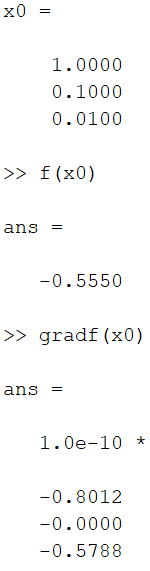
\includegraphics[scale = 0.9]{gamma10vals}
    \newline
    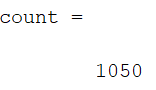
\includegraphics{gamma10count}
    \newline\newline
\end{center}

For $\gamma = 100$, we have $\text{cond}(Q) = 10000$ and the corresponding upper bound for the rate constant is $C = 0.999600$, so we expect even slower convergence. Using the script, we find it took 103,376 iterations to reach the tolerance $\|\nabla f(x_k) \| < 10^{-10}$.
\begin{center}
    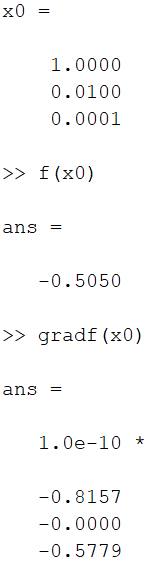
\includegraphics[scale = 0.9]{gamma100vals}
    \newline
    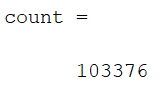
\includegraphics{gamma100count}
    \newline\newline
\end{center}

Finally, for $\gamma = 1000$, we have $\text{cond}(Q) = 10^6$ and the associated upper bound for the rate constant is given by $C = 0.999996$. Using the script, we find it took approximately 10.3 million iterations to reach the tolerance $\| \nabla f(x_k) \| < 10^{-10}$.
\begin{center}
    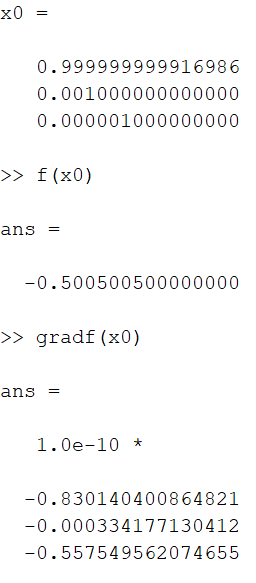
\includegraphics[scale = 0.9]{gamma1000vals}
    \newline
    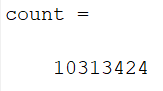
\includegraphics{gamma1000count}
    \newline\newline
\end{center}





\section*{Section 12.3 Problems}
\textbf{1.} Apply the symmetric rank-one quasi-Newton method to solve
\[\minimize \hspace{1em} f(x) = \frac{1}{2}x^TQx - c^Tx\]
with
\[Q = \begin{pmatrix}
    5 & 2 & 1\\
    2 & 7 & 3\\
    1 & 3 & 9
\end{pmatrix}
\hspace{1em} \text{and} \hspace{1em}
c = \begin{pmatrix*}[r]
    -9\\
    0\\
    -8
\end{pmatrix*}\]
Initialize the method with $x_0 = (0,0,0)^T$ and $B_0 = I$. Use an exact line search.
\newline\newline
Implementing the symmetric rank-one quasi-Newton method to solve the above problem with the given initial guesses, we find convergence after three iterations with the following values for the optimal point $x_*$, $f(x_*)$, and $\nabla f(x_*)$:
\begin{center}
    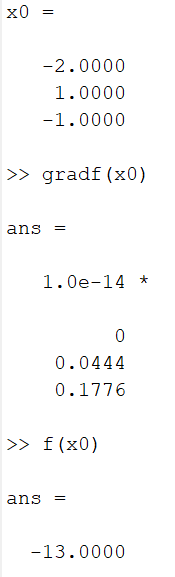
\includegraphics[scale = 0.9]{r1symVALS}
\end{center}
\textbf{2.}
Apply the BFGS quasi-Newton method to solve
\[\minimize \hspace{1em} f(x) = \frac{1}{2}x^TQx - c^Tx\]
with
\[Q = \begin{pmatrix}
    5 & 2 & 1\\
    2 & 7 & 3\\
    1 & 3 & 9
\end{pmatrix}
\hspace{1em} \text{and} \hspace{1em}
c = \begin{pmatrix*}[r]
    -9\\
    0\\
    -8
\end{pmatrix*}\]
Initialize the method with $x_0 = (0,0,0)^T$ and $B_0 = I$. Use an exact line search.
\newline\newline
Implementing the BFGS algorithm, we find convergence after three iterations with the following values for the optimal point $x_*$, $f(x_*)$, and $\nabla f(x_*)$:
\begin{center}
    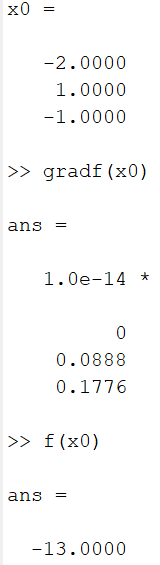
\includegraphics[scale = 0.9]{bfgsvals}
\end{center}


\textbf{4.} Let $C$ be a symmetric matrix of rank one. Prove that $C$ must have the form $C = \gamma ww^T$, where $\gamma$ is a scalar and $w$ is a vector of norm one.
\newline\newline
\textbf{Proof}: Let $C$ be a symmetric $n \times n$ matrix of rank one. Since $C$ is a rank one matrix, every row is a scalar multiple of one row of $C$. Call this the $i\text{th}$ row of $C$ and let $a_1, a_2, \cdots, a_n$ be scalars so that
\[C = \begin{pmatrix*}[c]
    a_1c_{i1} & a_1c_{i2} & \cdots & a_1c_{in} \\
    a_2c_{i1} & a_2c_{i2} & \cdots & a_2c_{in} \\
    \vdots & \vdots & & \vdots\\
    a_ic_{i1} & a_ic_{i2} & \cdots & a_ic_{i2} \\
    \vdots & \vdots & & \vdots\\
    a_nc_{i1} & a_nc_{i2} & \cdots & a_nc_{in} 
\end{pmatrix*}\]
Notice that we may rewrite the above expression for $C$ as
\[C = \mathbf{a}\mathbf{c}^T\]
with
\[\mathbf{a} = \begin{pmatrix*}
    a_1\\
    a_2\\
    \vdots\\
    a_n
\end{pmatrix*}
\hspace{1em}
\mathbf{c} = \begin{pmatrix*}
    c_{i1}\\
    c_{i2}\\
    \vdots\\
    c_{in}
\end{pmatrix*}\]
And since $C$ is symmetric, we have
\begin{align*}
    C^T &= (\mathbf{a}\mathbf{c}^T)^T\\
    &= \mathbf{c}\mathbf{a}^T\\
    &= \mathbf{a}\mathbf{c}^T
\end{align*}
Now, let $u\in \text{Im}(C)$ consider the following:
\begin{align*}
    Cu &= (\mathbf{ac}^T)u\\
    &= (\mathbf{c}^Tu)\mathbf{a}
\end{align*}
Let $k =\mathbf{c}^Tu$ so that $Cu = k\mathbf{a}$. Now consider
\begin{align*}
    C^Tu &= (\mathbf{ca}^T)u\\
    &= (\mathbf{a}^Tu)c
\end{align*}    
Let $l = \mathbf{a}^Tu$ so that $C^Tu = l\mathbf{c}$ and since $C^T = C$, we have
\begin{align*}
l\mathbf{c} &= k\mathbf{a}
\end{align*}
Since $u \in \text{Im}(C)$, we have $k, l \neq 0$ and so $\mathbf{a} = \alpha\mathbf{c}$ with $\alpha = l/k$. Then
\[C = \alpha\mathbf{c}\mathbf{c}^T\]
Now let $w = \frac{\mathbf{c}}{\|\mathbf{c}\|}$ so that $\|w\| = 1$ and $\gamma = \|\mathbf{c}\|^2\alpha$. We finally have
\[C = \gamma ww^T\]
which is what we sought to show.


\end{document}
